\documentclass[12pt]{article}
\usepackage{amssymb, amsthm, graphics, graphicx}
\usepackage{amsmath}

%these are initial settings. Ron recommended them, so that's just what I use.
\textwidth = 6.5 in
\textheight = 9 in
\oddsidemargin = 0.0 in
\evensidemargin = 0.0 in
\topmargin = -.75in
\parskip = 0.2 in
\parindent = 15 pt
\renewcommand{\baselinestretch}{1.25}

\providecommand{\e}[1]{\ensuremath{\times 10^{#1}}}
\providecommand{\degree}[0]{\ensuremath{^{\circ}}}

\providecommand{\ah}[1]{\ensuremath{\hat{a}_{#1}}}
\providecommand{\ahx}[0]{\ensuremath{\ah{x}}}
\providecommand{\ahy}[0]{\ensuremath{\ah{y}}}
\providecommand{\ahz}[0]{\ensuremath{\ah{z}}}
\providecommand{\pfs}[0]{\ensuremath{\epsilon_{0}}} %permittivity of free space => 1/(36\pi) \e{-9}
%\providecommand{\vec}[1]{\ensuremath{\textbf{#1}}} %vector notation ACTUALLY \vec is _real_ vector notation
\providecommand{\ohm}[0]{\ensuremath{\Omega}}
\providecommand{\jw}[0]{\ensuremath{j \omega}}


\newtheorem*{prob}{Problem}

\begin{document}
\begin{flushright}
\textbf{Charles Julian Knight}\\
ECE4893\\
\today
\end{flushright}


\begin{center}
\huge HW 4
\end{center}

\begin{prob}[1.a]{
Assume that the transductance gain of the OTA is $19.2*I_{con}$, where $I_{con}$ is the current flowing into the control pin of the OTA. What is the cutoff frequency of the filter block in terms of ($I_{con}$) in Hertz?
}\end{prob}
From our linear-region OTA equation, and using the input voltage divider $\frac{1k}{100k+1k}\approx .01$,

\[I_o = 19.1 I_{con}(0-.01 V_i)\]

This is then fed into the capacitor (as we assume the buffer input impedance is infinite). To avoid calculus, let's stay in the
frequency domain:

\[V_o = I_o Z_c = \frac{19.1 I_{con}(0-.01 V_i)}{\jw C} = \frac{-.191 I_{con}V_i}{\jw C}\]
Since the buffer is an ideal non-inverting, we can expect this to be the same on the other side. The transfer function is then
\[H(s) = \frac{1}{s \frac{C}{-.191I_{con}}}\]

where $\frac{C}{-.191I_{con}}$ is our ``kinda RC'' constant which defines our cutoff frequency.

\[f_o = \frac{.191I_{con}}{100p} = 1.91\e{9}I_{con} Hz \]

\begin{prob}[1.b]{
Given the result in (a), what value $I_{con}$ would be needed for the cutoff frequency of one stage to be 1000 Hz?
}\end{prob}
\[I_{con} = 1000/1.91\e{9} = 52.4 \mu A \]
This sounds too small. I expected something in the small mA range. I don't see any order-of-magnitude errors in my calculation though.

\begin{prob}[1.c]{
Now let's consider the full four-pole cascade with feedback level denoted as K, as in lecture. Let the cutoff frequency of a single stage be 1000 Hz. Using MATLAB, Mathematica, Maple, or some similar tool, on the same plot, show the magnitude of the frequency response (with the horizontal axis in Hertz), from DC to some value that you think best shows off the curves, for four cases: K=0, K just big enough so that you can just barely see a resonance ``bump'' in the curve, K close to 4 (but not so big that it swamps your other curves), and a K somewhere between the last two cases that you think is interesting.
}\end{prob}

Below are log-log plots (from 2Hz to 20KHz) of $K \in [0, .8, 3, 3.9]$. I used $0.8$ because, just as with second-order lowpass filters, the Butterworth response occurs at $K=.707$ so I picked a slightly larger value.  

\begin{center}
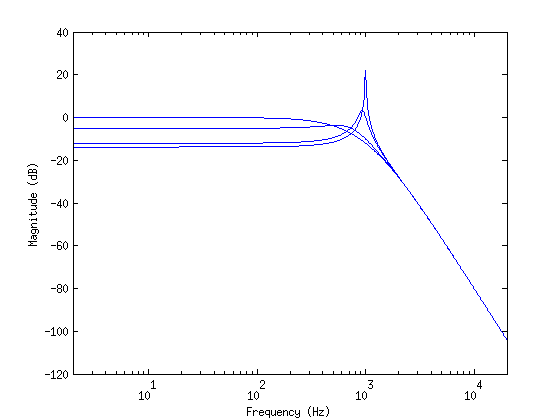
\includegraphics[width=5in]{graphs.png}
\end{center}

Below are the MATLAB-computed DC magnitudes for each K value. They agree with the expected $\frac{1}{1+K}$ to 4 decimal places.

\[ [1.0000, 0.5556, 0.2500, 0.2041] \]

%%%%%%%%%%%%%%%%%%%%%%%%%%%%%%%%%%%%%%%%%%%%%%%%%%%%%%%%%%%%%%%%%%%%%%%%%%%%%%%%%

\begin{prob}[2.a]{
Using this formula, find the cutoff frequency (in Hertz) of one of those sections in the Minimoog's transistor ladder as a function of the control current being pulled from the tied emitters of the transistor pair that feeds the ladder.
}\end{prob}

\[ f_c = \frac{1}{8\pi C V_T}I_f = (4.42\e{-8}HzA^{-1}) I_f \]

For a cutoff in the KHz range, this is again a control current in the 10s of $\mu A$ range.

\begin{prob}[2.b]{
Let's do some DC analysis. At DC, the caps are open circuits. For the purpose of this analysis, ignore R76 (the 330 ohm resistor) and the R73 (the 1K regeneration calibration pot); treat them as ``open'' too. Supposing that the transistors draw negligible current through the bases, what are the voltages at the bases of the four stages of the ladder? (Number the stages 1 through 4, from bottom to top; the first stage is Q23/Q24, the second is Q19/A20, the third is Q10/11, and the fourth is Q2/Q3).
}\end{prob}

At DC, we have a resistor ladder from $10V$ to ground: $[ 220\ohm, 150\ohm, 150\ohm, 150\ohm, 200\ohm ]$. The total is $870\ohm$.

\[ V_{b,stage1} = 10\frac{200}{870} = 2.30V \]
\[ V_{b,stage2} = 10\frac{350}{870} = 4.02V \]
\[ V_{b,stage3} = 10\frac{500}{870} = 5.75V \]
\[ V_{b,stage4} = 10\frac{650}{870} = 7.47V \]

%%%%%%%%%%%%%%%%%%%%%%%%%%%%%%%%%%%%%%%%%%%%%%%%%%%%%%%%%%%%%%%%%%%%%%%%%%%%%%%%%

\begin{prob}[3.a]{
Assuming a negative feedback factor of K, find the closed-loop transfer function of the complete filter. Write your answer so that it has $\omega_c^2$ in the numerator and a quadratic polynomial in s in the denominator. Make sure the highest power of s has unit coefficient, i.e. a coefficient of 1.
}\end{prob}
We can use the same equation for the four-pole version on the two-pole version, but updating the order:
\[ H_2(s) = \frac{\omega_c^2}{(s+\omega_c)^2 + K\omega_c^2} \]

\begin{prob}[3.b]{
 In class on March 5, we looked at a canonical lowpass 2nd-order filter transfer function of the form $\frac{\omega_n^2 }{s^2 + (\omega_n / Q) s + \omega_n^2}$, where $\omega_n$ was the ``natural frequency'' and Q was the ``quality factor.'' If you put your answer to (a) in this form, what are $\omega_n$ and Q in terms of $\omega_c$ and K?
}\end{prob}

\[ H_2(s) = \frac{\omega_c^2}{(s+\omega_c)^2 + K\omega_c^2} = \frac{\omega_c^2}{s^2+2\omega_cs + \omega_c^2 + K\omega_c^2} \]

\[ = \frac{\omega_c^2}{s^2+2\omega_cs + (1+K)\omega_c^2} \]

Thus, $\omega_n = \sqrt{1+K}\omega_c$ and $Q= \frac{1}{2\sqrt{1+K}}$.

\begin{prob}[3.c]{
What are $\omega_n$ and Q for the special case of K = 0 (i.e. no feedback)?
}\end{prob}
In this case, the equation simplifies to the normal 2nd order filter form, and $\omega_n=\omega_c$, and $Q=1/2$.

\begin{prob}[3.d]{
For what values of K does the filter exhibit a resonance bump, i.e. for what values of K is $Q > 1/\sqrt{2}$?
}\end{prob}

\[ Q = \frac{1}{2\sqrt{1+K}} > \frac{1}{\sqrt{2}} \]
\[ \frac{1}{4(1+K)} > \frac{1}{2}  \]
\[ 4(1+K) < 2 \]
\[ K < -2 \]

\begin{prob}[3.e]{
 Using the quadratic formula, find the locations of the poles of this filter as a function of $\omega_c$ and K.
}\end{prob}

\[ s_p = \frac{-(2)\pm \sqrt{2^2 - 4(1+K)}}{2} = \frac{-2\pm \sqrt{-K}}{2} \]

\begin{prob}[3.f]{
Where are the poles for the special case of K = 0?
}\end{prob}
\[ s_p0 = \frac{-2\pm \sqrt{0}}{2} = -1 \]
Thus, they are both at $-1$ (still on the real axis).

\begin{prob}[3.g]{
Describe how the poles move as K increases.
}\end{prob}

Using MATLAB, we can graph the poles for a few values. Below are plots for $K \in [-0.1, 0, .5]$. For negative values\footnote{Meaing positive feedback, I think? Nothing meaningful in the real world, in any case.} of K, the poles move along the real axis. At $K=0$ they meet, and above that they begin to move along the imaginary axis.

\begin{center}
% 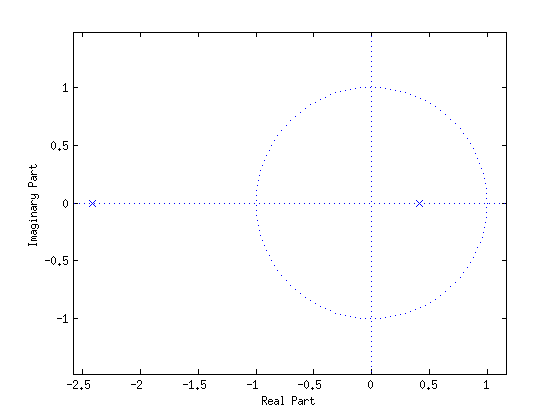
\includegraphics[width=2in]{k-2.png}
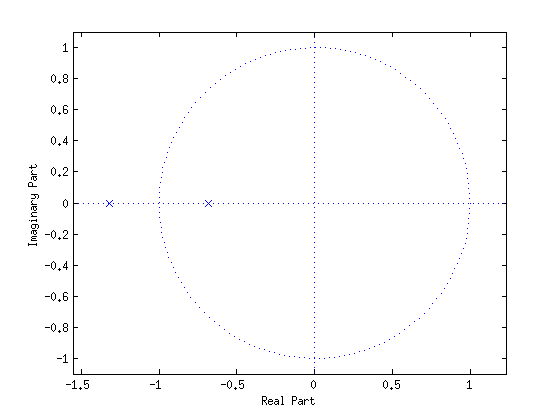
\includegraphics[width=2in]{k-01.png}
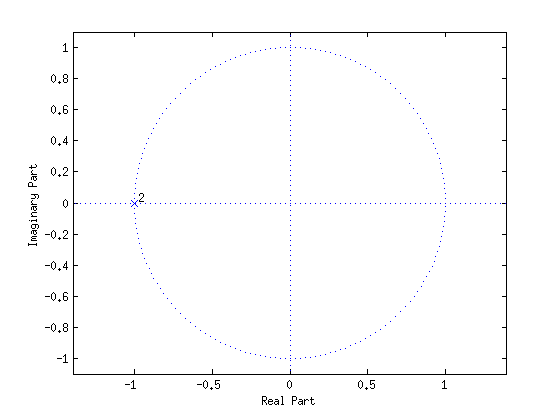
\includegraphics[width=2in]{k0.png}
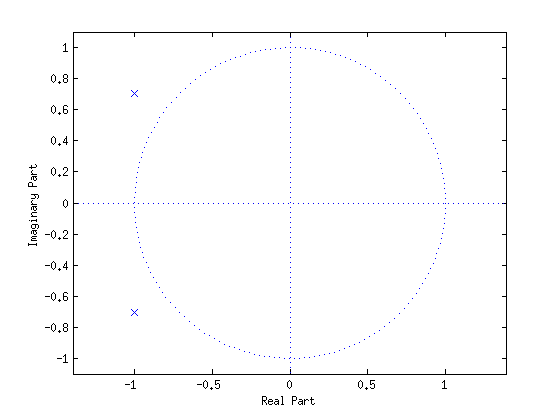
\includegraphics[width=2in]{k05.png}
% 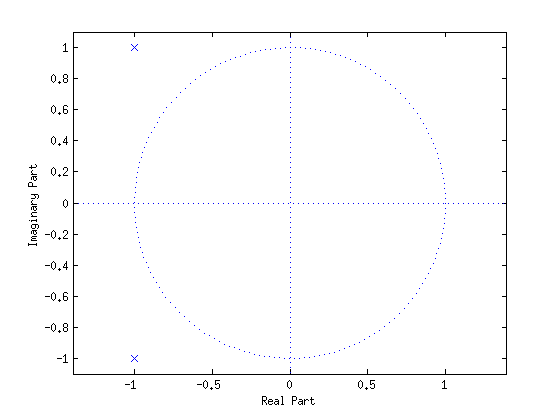
\includegraphics[width=2in]{k1.png}
\end{center}

\begin{prob}[3.h]{
Can this filter be made to self-oscillate like the four-pole-casade-with-feedback filter explored in the pervious problems? In other words, is there a value of $K > 0$ for which the poles can be made to lie on the imaginary axis?
}\end{prob}

No, because for $K>0$, the poles move only along the imaginary axis.

With negative values of K, one pole approaches the imaginary axis, and would cross at $K=-1$. But of course, if $K=-1$ then your $s^0$ term drops out and you loose an order and the pole disappears. Below are plots for $K \in [-0.9, -1, -11]$ to demonstrate.

\begin{center}
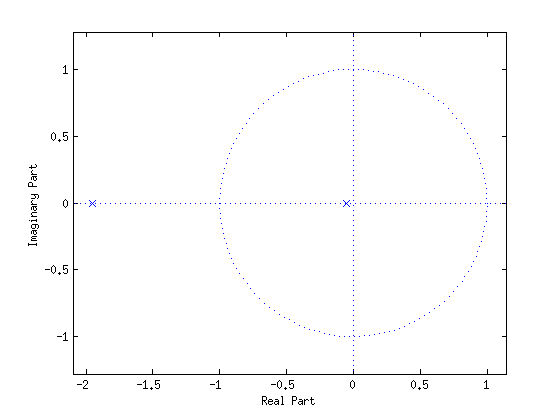
\includegraphics[width=2in]{k-09.png}
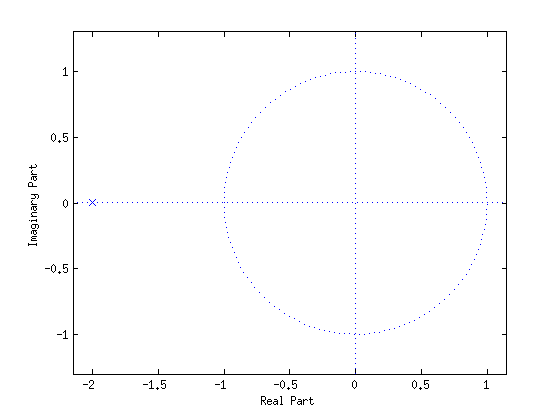
\includegraphics[width=2in]{k-1.png}
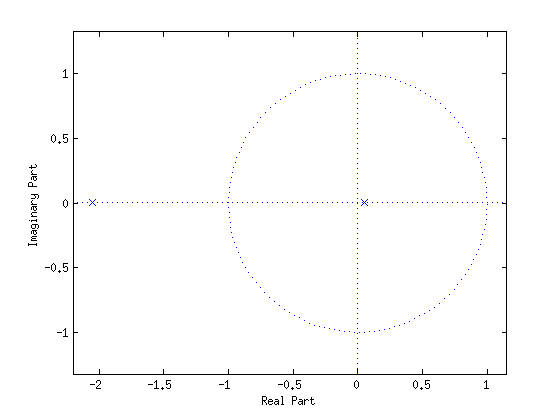
\includegraphics[width=2in]{k-11.png}
\end{center}

%\[ H(s) = \frac{\omega_c^2}{(s+\omega_c)^2 + K\omega_c^2}\frac{\omega_c^2}{(s+\omega_c)^2 + K\omega_c^2} \]

\end{document}
